\chapterimage{Intro/Intro_Figures/ArtisticView2.jpg} % Chapter heading image
%Einstein Telescope artists impression copyright Nikhef
%\section{Introduction}
\chapter{Introduction}
\label{chap:Intro}

%
% Extensive description of the document; history, table of the acronyms
%
% Author:
% Version:
%
\section[Prologue]{Prologue}
\label{Prologue}
The first generation of interferometric gravitational wave (GW) detectors  (GEO600~\cite{GEO600Grote2008}, LIGO~\cite{Abbott2009}, TAMA~\cite{Arai2008}, Virgo~\cite{VirgoStatus2008}) have reached or approached their design sensitivities, and thus demonstrated the effectiveness of the working principle. 
The major detectors currently operative are enhanced versions of the first generation (Virgo+ and eLIGO), with higher laser power and some technological improvements.

Advanced detectors (like ``Advanced LIGO"\,(\cite{AdvancedLIGOReference2009},\,\cite{aLIGO}) and ``Advanced Virgo" \,(\cite{AdV2009})), also called the second generation, will show a sensitivity improved roughly by a factor of ten with respect to the initial interferometers. They are based on technologies currently available, sometimes tested in reduced scale prototypes, but still to be implemented in full scale. 
According to the current models of GW sources, the sensitivity of the advanced interferometers is expected to guarantee the detection of signals generated by astrophysical sources within months to a year at most. For example, at the nominal sensitivity of the advanced detectors, the expected detection rate of the GW signal generated by a binary system of coalescing neutron stars is about a few tens per year. But apart from extremely rare events, the expected signal-to-noise ratio (SNR) of these detections obtained with the advanced detectors is too low for precise astronomical studies of the GW sources and for complementing optical and X--ray observations in the study of fundamental systems and processes in the Universe.

These considerations led the GW community to start investigating a new (third) generation of detectors. In particular, the European Commission supported the institutions in Table~\ref{table:Beneficiaries} to realise this design study within the Seventh Framework Programme (FP7-Capacities). With a considerably 
improved sensitivity, such new machines of the third-generation will open the era of routine GW astronomy and with the Einstein Telescope (ET) project Europe will lead this scientific revolution. Since the first detection of a GW signal is expected to occur in the advanced interferometers, the evaluation of the scientific impact of ET it is especially focused on the observational aspects rather than on the detection capabilities.

To realise a third-generation GW observatory with a significantly enhanced sensitivity (we defined a target of a factor of ten improvement in sensitivity for ET with respect to the advanced detectors over a wide frequency range), several limitations of the technologies adopted in the advanced interferometers must be overcome and new solutions to be developed are proposed in this document to reduce the fundamental and technical noises that will limit the next generation machines. \par

the first and main target of this document is the definition of 
the requirements and of the main characteristics of the site hosting ET, 
the design of the key elements of the research infrastructure, the rough 
evaluation of the costs and of the timeline of its implementation.  To 
understand the importance and the need of the site and infrastructures 
in the ET design it is worth to recall the history of the current GW detector 
infrastructures, shown in Fig.~\ref{Fig:InfraEvolution}.

Current and advanced detectors are using the same infrastructure that 
will be about 20 years old when the second generation will be online. 
Further improvements of the sensitivity will be limited by the constraints 
of the site and infrastructure (arm length, local seismic noise, absence of 
cryogenic apparatus, vacuum pipe size\,\ldots). Indeed, in order to realise 
a third-generation GW observatory like ET, an infrastructure hosting 
several detectors that evolve for many decades is crucial.


\begin{figure*}
\centering
\includegraphics[width=0.99\textwidth]{Intro/Intro_Figures/GWDAW-2010PunturoInfrastructureAdv.png}
%\includegraphics[width=0.9\textwidth, bb=0 0 800 600]{Sec_Introduction/GWDAW-2010PunturoInfrastructureAdv.png}
%\includegraphics[width=0.49\textwidth, bb=0 0 800 600]{ET-B.png}
\caption{Evolution of the first and second generation GW detectors. Time is on the horizontal axis, detector performance in the vertical one. When the advanced detectors will be operative the hosting infrastructures will be more than 20 years old and any further improvement of performance (sensitivity) will be suppressed by the limitation imposed by the infrastructures. (slide presented by M.\,Punturo at the GWDAW meeting, Rome Jan.\,2010).}
\label{Fig:InfraEvolution}
\end{figure*}